\documentclass[12pt]{article}

\usepackage{sbc-template}
\usepackage{graphicx,url}
\usepackage{tikz} 
\usetikzlibrary{automata, arrows, positioning}

\usepackage{mathtools}
\usepackage{amssymb}
\usepackage{amsmath}
\usepackage{algorithm}
\usepackage[noend]{algpseudocode}

\usepackage{listings}
\usepackage{xcolor}

\usepackage[utf8]{inputenc}

\makeatletter
\def\BState{\State\hskip-\ALG@thistlm}
\makeatother

\definecolor{codegreen}{rgb}{0,0.6,0}
\definecolor{codegray}{rgb}{0.5,0.5,0.5}
\definecolor{codepurple}{rgb}{0.58,0,0.82}
\definecolor{backcolour}{rgb}{0.95,0.95,0.92}

\lstdefinestyle{mystyle}{
    commentstyle=\color{codegreen},
    keywordstyle=\color{magenta},
    numberstyle=\tiny\color{codegray},
    stringstyle=\color{codepurple},
    basicstyle=\ttfamily\footnotesize,
    breakatwhitespace=false,         
    breaklines=true,                 
    captionpos=b,                    
    keepspaces=true,                 
    numbers=left,                    
    numbersep=5pt,                  
    showspaces=false,                
    showstringspaces=false,
    showtabs=false,                  
    tabsize=2
}

\lstset{style=mystyle}
     
\sloppy

\title{Estudo de diferentes formas de enumeração de ciclos em um grafo}

\author{Gustavo Lopes Rodrigues\inst{1}, Thiago Henriques Nogueira\inst{2},}


\address{Instituto de Ciências e Informática \\Pontifícia Universidade Católica de Minas Gerais
  (PUC-MG)\\}


\begin{document} 

  \maketitle

  \begin{abstract} 
    This document serves as a report on the study in two different ways
    to enumerate cycles within a graph: permutation and walking. For this
    study, we only work with non-directed graphs. In order to test the effiency 
    of both algorythms,we also implemented a method to calculate the performance of walking
    X permutation as the graph increases.
  \end{abstract}

  \begin{resumo} 
    Este documento serve como um relatório sobre o estudo em duas maneiras 
    diferentes de enumerar ciclos dentro de um grafo: permutação e por caminhamento. Para esse 
    estudo, trabalhamos apenas com grafos não-direcionados. Então fizemos um método
    para calcular o desempenho do caminhamento e da permutação, na medida que o grafo aumentasse.
  \end{resumo}


  \section{Informações gerais}

    Este é um trabalho feito para a disciplina de Algoritmo em Grafos, para a 
    \emph{Pontifícia Universidade Católica de Minas Gerais}, onde foi necessário 
    implementar duas maneiras diferentes de enumerar todos os ciclos dentro de um 
    grafo não direcionado: permutação e caminhamento. O objetivo final  deste relatório, 
    é de descrever toda a implementação do grafo e da resolução do problema, assim como 
    comparar ambos os algoritmos em questão do desempenho.

    Na seção \ref{sec:graph}, detalhamos a estrutura de grafo que foi usada para essa atividade,
    assim também como os seus principais componentes. Em \ref{sec:permutation} e \ref{sec:walking},
    detalhamos como implementos os nossos algoritmos de permutação e caminhamento respectivamente.
    A seção \ref{sec:performance} é a demonstração da performance dos códigos, assim como também 
    os grafos utilizados para os testes e como fizemos os testes. Por fim, na seção \ref{sec:conclusion}
    concluímos o trabalho com nossas perspectivas sobre os resultados.

  \section{Grafo} \label{sec:graph}

    Para maior organização, todas as classes implementadas possuem um header (arquivo .hpp)
    e o grafo não é uma exceção. Em graph.hpp é colocado todas as variáveis, assim também como as 
    funções usadas pelo grafo. Em graph.cpp, todas as declarações feitas no arquivo .hpp, são 
    implementadas.
    
    Para o nosso próposito, apenas duas estruturas foram usadas para guardar informações sobre
    o grafo: primeiro temos um vetor , com um vetor de indíces. A ideia é colocar listas flexíveis,
    onde cada posição representa os adjacentes de determinado vértice. Essa estrutura é muito
    importante para a permutação. 

    \begin{lstlisting}[language=c++]
      
      std::vector<std::vector<counter>> adj;
    \end{lstlisting}

    Para o caminhamento, utilizamos também um vetor, porém um vetor com um par(std::pair): 
    o primeiro é o peso, o segundo é outro par, porém este possui a vértice de entrada(source)
    e destino(destination). Basicamente esta estrutura guarda as relações entre as arestas 
    do grafo, assim como o peso dessas relações.

    \begin{lstlisting}[language=c++]
      
      std::vector<std::pair<weight,std::pair<counter,counter>>> edges_weights;
    \end{lstlisting}

    Os outros dois atributos referem-se apenas aos contadores de vértices e arestas.

    Com todos os atributos mencionados, agora vamos para as principais funções do grafo:

  \subsection{Construtores} \label{ssec:constructors}

    Nosso grafo possui três construtores:

    \begin{itemize}
      \item O primeiro apenas inicia o grafo, sem nenhum vértice. 
      \item O segundo construtor inicia o grafo com N número de vértices, porém, sem arestas,
      logo é criado um grafo nulo.
      \item O terceiro construtor foi feito para a realização dos testes. Ele pega informações do
      grafo a partir de um arquivo .txt, sendo a primeira linha o número de vértices e as linhas 
      seguintes contendo as arestas, assim como os pesos(se tiver).
    \end{itemize}

  \subsection{getters}

    Depois dos construtores, temos as funções do tipo getters, que retornam a quantidade de vértices 
    e de arestas dentro do grafo.

  \subsection{add\_vertex}

    Finalmente, começando com as funcionalidades do grafo, temos a função para adicionar 
    uma vertex isolada ao grafo, adicionando um iterator ao vetor. Se a operação for um sucesso, 
    será retornado o index do vértice adicionado.

  \subsection{add\_edge}

    Se houver os vértices especificados, será adicionado a nova ligação a lista de 
    adjacência e de arestas. Se o peso não for especificado, ele será colocado como zero.
    Por fim, a função retorna um booleano, indicando se foi um sucesso.

  \subsection{print}

    A função print é responsável em imprimir o atual estado do grafo, tanto
    em questão das adjacências, quanto as arestas e seus pesos respectivamente.

  \section{Permutação} \label{sec:permutation}

    Com as funcionalidades gerais do grafo especificadas, é possível agora ir para a 
    implementação do algoritmo de permutação. Na teoria de grafos, permutação significa
    percorrer por todos os vértices uma única vez,seguindo a ordem: [v1,a1,v2,a2...]

    O algoritmo de permutação escolhido foi o busca em profundidade(também conhecido 
    como DFS(Depth-first-search)), a ideia do algoritmo é percorrer todos os vértices,
    com o intuito de achar o vértice mais fundo.
    
    Em nossa implementação, o vértice inicial sempre será o "vértice raiz"(index 0), 
    e para memorizar todos os vértices já visitados, também é utilizado um vetor de cores,
    onde o seu tamanho é igual ao número de vértices, e cada posição representa um vértice do 
    grafo. Eis as cores utilizadas e seus significados:

    \begin{itemize}
      \item WHITE: Vértice e sua vizinhança ainda não visitado.
      \item YELLOW: Vértice visitado porém não sua vizinhança como todo.
      \item RED: Vértice visitado assim como sua vizinhança.
    \end{itemize}

    Por fim, vamos dar uma olhada em quais são os passos que o código 
    faz, para chegar ao resultado desejado:

    \begin{algorithm}
      \caption{Permutation} \label{euclid}
      \begin{algorithmic}[1]
      \Procedure{DFS}{}
      \State {$\text{colors} \gets \text{[G.vertex]}$}
      \For{$\text{v in G.V}$}
      \If{$\text{colors[v] == WHITE}$}
      \State {$\textbf{visit(v,colors)}$}
      \EndIf
      \EndFor
      \EndProcedure
      \Procedure{visit}{index,colors}
      \State {$\text{colors[index]} \gets \text{YELLOW}$}
      \For{$\text{v in G.adj[index]}$}
      \If{$\text{colors[v] == WHITE}$}
      \State {$\textbf{visit(v,colors)}$}
      \EndIf
      \EndFor
      \State {$\text{colors[index]} \gets \text{RED}$}
      \EndProcedure
      \end{algorithmic}
    \end{algorithm}

    A esquemática acima define como é normalmente o código para a busca em profundidade. 
    Para adaptar de forma que ela consiga encontrar ciclos, precisamos enviar para a 
    função \emph{visit}, o pai do vértice, e verificar se o vértice que está sendo visitado 
    está com a cor \emph{AMARELO} e este não é o pai.

  \section{Caminhamento} \label{sec:walking}

  Caminhamento é uma sequência de vértices e arestas de um grafo. Ao atravessar um grafo,
  um caminhamento ocorre e tanto vértices quanto arestas podem ser repetidas neste processo.

  Existe diferentes tipos de caminhamento, porém, para os objetivos desse relatório, isto 
  é o suficiente para entender como implementamos o nosso algoritmo escolhido, que no caso 
  é o de Kruskal.

  O algoritmo de Kruskal, inventado pelo matemático Joseph Kruskal, foi feito para buscar 
  uma árvore geradora mínima(Minimum Spanning Tree), em um grafo conexo e que possua pesos. 
  Então fica a pergunta: se o Kruskal serve para encontrar uma MST, então como podemos usa-lo 
  para encontrar ciclos? 

  Para responder essa pergunta, precisamos entender a lógica do algoritmo:

  \begin{algorithm}
    \caption{Walk} \label{euclid2}
    \begin{algorithmic}[1]
    \Procedure{Kruskal}{}
    \State {$\text{T} \gets \varnothing$}
    \State {$\text{queue} \gets \text{sort (u, v) edges of E using 1}$}
    \For{$\text{v in G.V}$}
    \State {$\text{make-tree(v)}$}
    \EndFor
    \While{$\text{queue} \neq \varnothing \text{ AND trees-count $>$ 1}$}.
    \State {$\text{\{u,v\}} \gets \text{queue.extractMin()}$}
    \If{$\text{!(T } \cup \text{(\{u, v\} has cycle)}$}
    \State {$\text{T.add(\{u,v\})}$}
    \State {$\text{merge (tree-of(u), tree-of(v))}$}
    \EndIf
    \EndWhile
    \EndProcedure
    \end{algorithmic}
  \end{algorithm}

  Para a realização do Kruskal, ele necessita fazer a verificação caso um ciclo seja formado
  ao unir as duas arestas. Por isso, adicionar mais uma verificação e um contador é o suficiente 
  para que seja possível contar o número de ciclos.

  Além disso, adicionamos uma estrutura auxiliar. O Disjoin-sets é uma estrutura separada do grafo,
  que foi criada para ser utilizada apenas no Kruskal. O objetivo de se utilizar Disjoin-sets é para 
  manter o controle dos vértices particionadas em subconjuntos, e então juntá-las a medida que for necessário.

  \section{Desempenho} \label{sec:performance}

  Com a explicação dos grafos deixada de lado, agora será explicado como foi feito os testes de performance.

  Na seção \ref{ssec:constructors}, foi detalhado os construtores do grafo. Entre eles,
  o construtor 3 do grafo foi feito especificamente para realização dos testes. Ele 
  recebe um char* com o diretório de um arquivo ".txt". Esse arquivo possui informações como número de 
  vértices, as relações entre os vértices, e por fim, se tiver, o peso das arestas.

  Para iniciar o programa, o usuário precisa enviar parâmetros para a função, entre esses parâmetros estão:

  \begin{itemize}
    \item A quantidade de testes a ser feito.
    \item Qual método de contagem de ciclo usar ("kruskal" ou "dfs").
    \item O diretório para os arquivos com os grafos.
  \end{itemize}

  Ao iniciar o programa com os parâmetros necessários, um número 'n' do teste especificado 
  será realizado nos grafos inseridos, e o resultado será colocado em um arquivo("results.txt").

  Antes de mostrar os testes, também gostaria de colocar as especificações do computador 
  que foi utilizado para a realização dos testes, pois isso pode ser também um fator 
  que influência nos tempos alcançados.

  OS: Arch Linux
  
  KERNEL: 5.12.2-arch1-1
  
  CPU: Intel Core i7-7700 @ 3.60GHz
  
  GPU: NVIDIA GeForce GTX 1060 6GB
  
  RAM: 16 GB
  
  A seguir terá subseções divididas em: esquemática do grafo, assim como 
  uma tabela com informações sobre o teste: número de testes, algoritmo e
  tempo médio.

  \subsection{Grafo 1}

  \begin{figure}[ht]
    \centering
    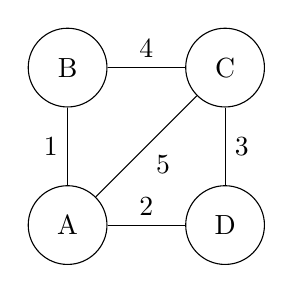
\begin{tikzpicture}[node distance = 3cm,  auto,main/.style = {draw, circle,minimum size=10mm}] 
      \node[main] (1) at (0,0) {A}; 
      \node[main] (2) at (0,2)  {B}; 
      \node[main] (3) at (2,2)  {C};
      \node[main] (4) at (2,0)  {D};


      \path[-]
      (1) edge              node {1} (2)            
      (2) edge              node {4} (3)
      (3) edge              node {3} (4)
      (3) edge              node {5} (1)
      (1) edge              node {2} (4);
    \end{tikzpicture} 
    \caption{Grafo \arabic{subsection} - 4 vértices e 5 arestas }

  \end{figure}

  \begin{table}[htbp]
    \caption{Testes nos algoritmos implementados usando o grafo \arabic{subsection}}
    \begin{center}
    \begin{tabular}{|c|c|c|c|}
    \hline
    \textbf{Número de}&\multicolumn{2}{|c|}{\textbf{Tempo médio(em segundos)}} \\
    \cline{2-3} 
    \textbf{testes} & \textbf{\textit{DFS}}& \textbf{\textit{Kruskal}} \\
    \hline
    10$^{\mathrm{1}}$& 0.0363 & 0.0051 \\
    \hline
    10$^{\mathrm{2}}$& 0.01504 & 0.00534 \\
    \hline
    10$^{\mathrm{3}}$& 0.010091 & 0.003813 \\
    \hline
    10$^{\mathrm{4}}$& 0.0097517 & 0.0033486 \\
    \hline
    10$^{\mathrm{5}}$& 0.00973527 & 0.00333444 \\
    \hline
    \textbf{Média total:} & 0.08091797 & 0.02093604 \\
    \hline
    \end{tabular}
    \end{center}
  \end{table}

  Uma das coisas que pode ser observado nesse teste e nos próximos, é de que: a medida que 
  mais testes são feitos, o tempo médio vai ficando cada vez mais preciso. De qualquer maneira,
  é possível observar uma coisa bem interessante nessa tabela, no começo, o DFS(busca em profundidade)
  começa com um desempenho um pouco melhor do que o Kruskal, porém, com os testes seguintes, 
  o DFS fica com um desempenho 4x pior que o Kruskal.

  \newpage

  \subsection{Grafo 2}

  \begin{figure}[ht]
    \centering
    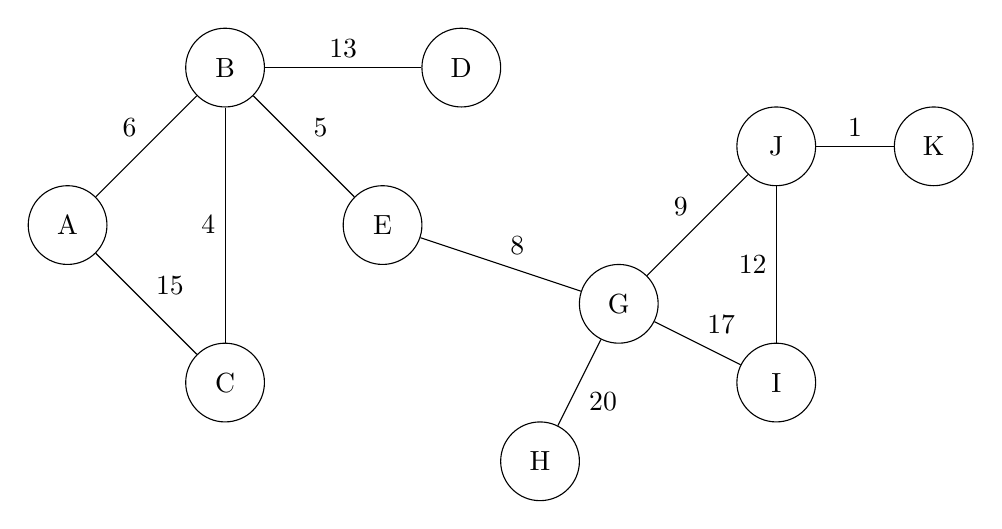
\begin{tikzpicture}[node distance = 3cm,  auto,main/.style = {draw, circle,minimum size=10mm}] 
      \node[main] (1) at (-10,5) {A}; 
      \node[main] (2) at (-8,7)  {B}; 
      \node[main] (3) at (-8,3)  {C};
      \node[main] (4) at (-5,7)  {D};
      \node[main] (5) at (-6,5)  {E}; 
      \node[main] (6) at (-3,4)  {G};   
      \node[main] (7) at (-4,2)  {H};   
      \node[main] (8) at (-1,3)  {I};  
      \node[main] (9) at (-1,6) {J};        
      \node[main] (10) at (1,6)  {K};  

      \path[-]
      (1) edge              node {6}  (2)            
      (1) edge              node {15} (3)
      (3) edge              node {4}  (2)
      (2) edge              node {13} (4)
      (2) edge              node {5}  (5)
      (5) edge              node {8}  (6)
      (6) edge              node {20} (7)
      (6) edge              node {17} (8)
      (6) edge              node {9}  (9)
      (8) edge              node {12} (9)
      (9) edge              node {1}  (10);
    \end{tikzpicture} 
    \caption{Grafo \arabic{subsection} - 10 vértices e 11 arestas }

  \end{figure}

  \begin{table}[htbp]
    \caption{Testes nos algoritmos implementados usando o grafo \arabic{subsection}}
    \begin{center}
    \begin{tabular}{|c|c|c|c|}
    \hline
    \textbf{Número de}&\multicolumn{2}{|c|}{\textbf{Tempo médio(em segundos)}} \\
    \cline{2-3} 
    \textbf{testes} & \textbf{\textit{DFS}}& \textbf{\textit{Kruskal}} \\
    \hline
    10$^{\mathrm{1}}$& 0.0566 & 0.0186 \\
    \hline
    10$^{\mathrm{2}}$& 0.02091 & 0.01429 \\
    \hline
    10$^{\mathrm{3}}$& 0.015381 & 0.010599 \\
    \hline
    10$^{\mathrm{4}}$& 0.0155222 & 0.0104494 \\
    \hline
    10$^{\mathrm{5}}$& 0.0154798 & 0.0103009 \\
    \hline
    \textbf{Média total:} & 0.123893 & 0.0642393 \\
    \hline
    \end{tabular}
    \end{center}
  \end{table}

  Com o aumento do número de vértices e arestas, também há como esperado um aumento no tempo médio para rodar 
  ambos os algoritmos. Entretanto, é interessante notar que a diferença entre o DFS e o Kruskal ficou menor, agora 
  o Kruskal é só 2x melhor do que o DFS.

  \newpage

  \subsection{Grafo 3}

  \begin{figure}[ht]
    \centering
    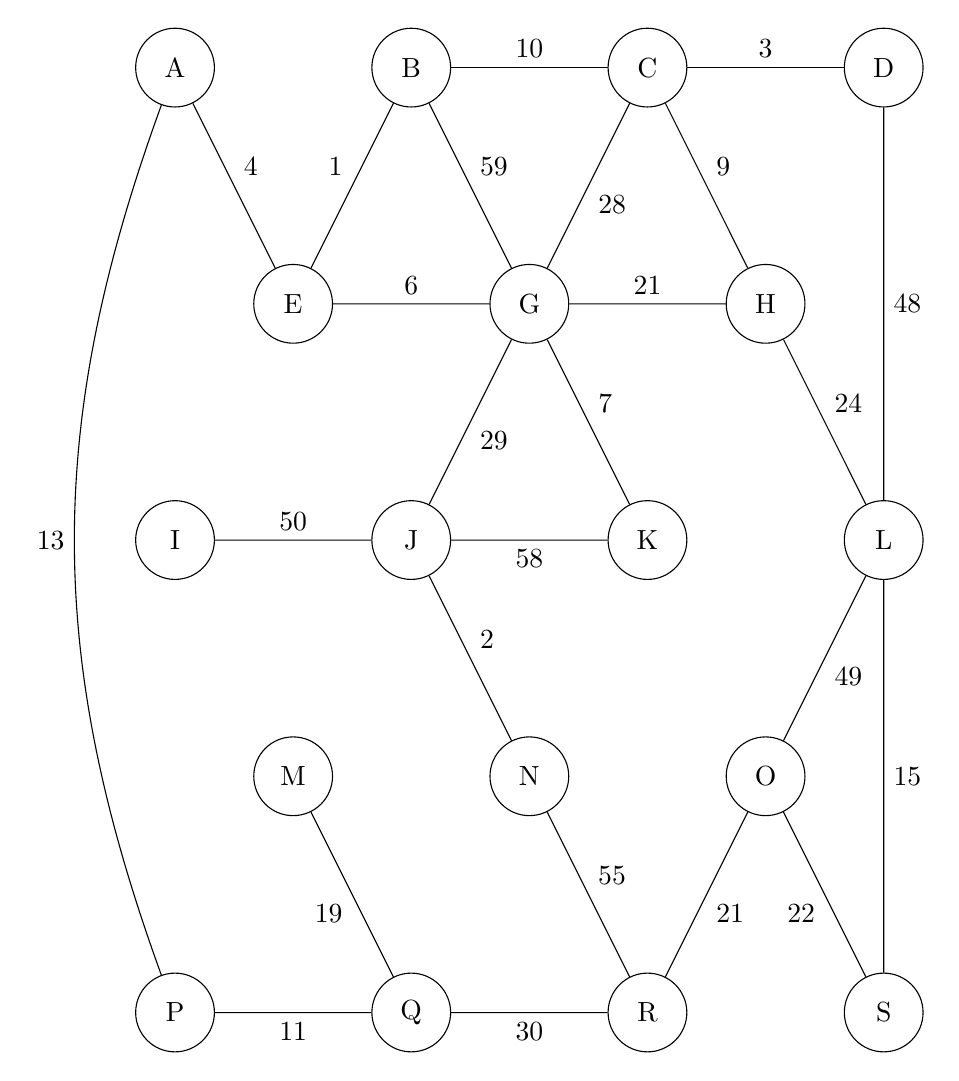
\begin{tikzpicture}[scale=1.5,node distance = 3cm, auto, main/.style = {draw, circle,minimum size=10mm}] 
      \node[main] (1) at (0,0)   {A}; 
      \node[main] (2) at (2,0)   {B}; 
      \node[main] (3) at (4,0)   {C};
      \node[main] (4) at (6,0)   {D};
      \node[main] (5) at (1,-2)  {E}; 
      \node[main] (6) at (3,-2)  {G};   
      \node[main] (7) at (5,-2)  {H};   
      \node[main] (8) at (0,-4)  {I};   
      \node[main] (9) at (2,-4)  {J}; 
      \node[main] (10) at (4,-4)  {K};  
      \node[main] (11) at (6,-4)  {L};   
      \node[main] (12) at (1,-6)  {M}; 
      \node[main] (13) at (3,-6)  {N};   
      \node[main] (14) at (5,-6)  {O};  
      \node[main] (15) at (0,-8)   {P}; 
      \node[main] (16) at (2,-8)   {Q}; 
      \node[main] (17) at (4,-8)   {R};
      \node[main] (18) at (6,-8)   {S};

      \path[-]
      (1)  edge                 node {4}  (5)
      (5)  edge                 node {1}  (2)
      (2)  edge                 node {10}  (3)
      (3)  edge                 node {3}  (4)
      (5)  edge                 node {6}  (6)
      (6)  edge                 node {21}  (7)
      (2)  edge                 node {59}  (6)
      (3)  edge                 node {28}  (6)
      (3)  edge                 node {9}  (7)
      (4)  edge                 node {48}  (11)
      (7)  edge                 node {24}  (11)
      (11) edge                 node {15}  (18)
      (6)  edge                 node {7}  (10)
      (10) edge                 node {58}  (9)
      (6)  edge                 node {29}  (9)
      (8)  edge                 node {50}  (9)
      (11) edge                 node {49}  (14)
      (14) edge                 node {21}  (17)
      (9)  edge                 node {2}  (13)
      (13) edge                 node {55}  (17)
      (17) edge                 node {30}  (16)
      (16) edge                 node {11}  (15)
      (15) edge [bend left=20]  node {13}  (1)
      (16) edge                 node {19}  (12)
      (18) edge                 node {22}  (14);

    \end{tikzpicture} 
    \caption{Grafo \arabic{subsection} - 18 vértices e 26 arestas }
  \end{figure}

  \begin{table}[htbp]
    \caption{Testes nos algoritmos implementados usando o grafo \arabic{subsection}}
    \begin{center}
    \begin{tabular}{|c|c|c|c|}
    \hline
    \textbf{Número de}&\multicolumn{2}{|c|}{\textbf{Tempo médio(em segundos)}} \\
    \cline{2-3} 
    \textbf{testes} & \textbf{\textit{DFS}}& \textbf{\textit{Kruskal}} \\
    \hline
    10$^{\mathrm{1}}$& 0.0877 & 0.0469 \\
    \hline
    10$^{\mathrm{2}}$& 0.02977 & 0.0287 \\
    \hline
    10$^{\mathrm{3}}$& 0.024836 & 0.025789 \\
    \hline
    10$^{\mathrm{4}}$& 0.0251404 & 0.0253671 \\
    \hline
    10$^{\mathrm{5}}$& 0.025174 & 0.0250916 \\
    \hline
    \textbf{Média total:} & 0.1926204 & 0.1518477 \\
    \hline
    \end{tabular}
    \end{center}
  \end{table}

  \newpage

  Por fim, temos mais um resultado interessante. Começou com o Kruskal tendo um desempenho 
  significativamente maior, e com o aumento do número de vértices e de arestas, a diferença entre 
  os dois foi diminuindo e com este grafo não é diferente. Com 10$^{\mathrm{5}}$ testes, a diferença 
  entre os dois é quase inexistente.
  
  \section{Conclusão} \label{sec:conclusion}

  No ínicio deste trabalho, acreditavamos que o DFS teria um desempenho melhor, devido ao fato que
  ele realiza uma permutação no grafo, logo, só irá passar uma única vez pelos vértices. Entretanto 
  na maioria dos casos o Kruskal conseguia um desempenho melhor, sendo apenas no final o momento que 
  ambos começaram a apresentar um desempenho equivalente.

  Essa diferença começa a fazer mais sentido, quando colocado em perspectiva com a complexidade
  de ambos os algoritmos. Kruskal possui uma complexidade de O(e*log(e) + e*log(v)) enquanto que 
  a busca em profundidade possui uma complexidade de O(v + e). Isso deixa claro o fato que quando 
  você possui um grafo denso(com muitas arestas), acaba que o custo da operação fica mais alto, logo, 
  explicando o comportamento dos algoritmos durante os testes.

\end{document}